Introduction to the implementation section

\section{Language and environment}

To understand what programming language and environment will be best suited for this project, I first  provide the technical requirements that will need to be met. The programming language will need to be  relatively fast when processing the rules of the L-systems and when rewriting these strings according to those rules. \\
\\
The program will also need to interpret the strings generated by the L-system rules and be able to generate a three dimensional representation of that L-system. This representation will need to be intuative and will have to allow me to examine it from different perspectives. In order to make the representation intuative, the 3D representation should be rendered in real time at multiple frames per second. And the user should be able to use a computer mouse and keyboard to move around the 3D world. \\ 
\\
Due to these demands have decided to use the C and C++ programming language. Due to its and thoroughly tested in built standard template library, I can count on it to be reliable and fast enough for the purpose of this project. It will also allow me to use other very useful libraries for 3D graphics such as \gls{OpenGL} which is also written in \GLS{C/C++}. I will be speaking in more detail about these details of these libraries in later sections. \\
\\
In order to create a window and provide the environment for writing pixels to the screen I will make use of the Graphics Library Framework (\acrshort{glfw}). Some useful mathematics functions and facilities can be found in the \gls{OpenGL} Matematics Library (\acrshort{glm}) and possibly the most important for rendering in 3D is the Open Graphics Library or \gls{OpenGL} for short. All of these libraries together will provide me with a strong foundation of tools that I can use to approach the practical aspect of this project. \\
\\
 

\subsection{C/C++ Programming Language}

The C programming language developed by Dennis Richie and Bell Labs in 1972 has been one of the most popular programming languages for a number of decades now \cite{ritchie1975c}. The C language was then extended upon by Bjarne Stroustrup in 1985 to create the C++ programming language \cite{stroustrup2000c++}. I have included both C and C++ as the programming languages that I will be using, as they are very closely related and C code can be compiled using the C++ compiler. For the most part I will be writing C++ code and making use of its object oriented features. However, their are instances when it will be more convenient to write C code or make use of a C library. 

\subsection{Standard Template Library (\acrshort{stl})}

The \acrshort{stl} in C/C++ provides a number of useful functions, data structures and algorithms that have been extensively tested for both reliability and efficiency. The most common features I will be using are strings, vectors, stacks and input and output. It is possible that in some cases it may be more efficient to use custom data structures for the most part the \acrshort{stl} functions will be more than good enough. \cite{horton2015stl} 

\subsection{Open Graphics Library (OpenGL)}

\gls{OpenGL} is a 2D and 3D graphics \acrshort{api}

talk about \acrshort{glsl}
\cite{movania2017opengl}

\subsection{OpenGL Mathematics Library ( \acrshort{glm} )}

\subsection{Graphics Library Framework(\acrshort{glfw})}

\subsection{Git Version Control}
Git is a free and open source version control software, that is able to keep track of changes that have been made to the files within a project folder. It will be used to keep track of previous versions of the project throughout the development process. Git can be used in conjuction with Github, which is a online web application that stores git repositories. This acts as a backup as well as containing all previous versions of the project.


\section{L-system Generator} \label{l-system generator section}

The purpose of the L-system generator is to read a file, called the L-system discriptor which contains any information that might be necessary for the string rewriting process. This file must contain the number of times the string will be rewritten (number of generations), a starting point (axiom) and at least one production rule, it may also contain some constant variables and other information. \\
\\
For simple L-systems, the generator need not be too complicated. The Koch Curve L-system stated below is a good example of this. \\
\\
\textbf{Angle:} 90\\
\textbf{Axiom:} F\\
\textbf{Rules:} \\
F $\rightarrow$ F+F-F+F\\
\\
Here we have a constant value of 90 degrees, the starting point of 'F' and one rule F $\rightarrow$ F+F-F+F. This type of system is very simple to rewrite computationally. \\ 
\\
\textbf{\textit{Here we describe some pseudocode}}\\
\\
When we move onto some more complicated L-systems, such as those that use parameters which have expressions with both variables and numbers. We end up with an L-system file that is quite difficult to process and rewrite. In order to compute these complex L-systems we need to first develop a formal grammar that describes how L-system files are defined. Once we have a formalization of how to define an parametric l-system we can create a system to carry out the rewriting.

\subsection{Building a Generalised L-system Grammar}

We are now able to represent complex three dimensional tree structures in the form of a L-system rule set. In a computing sense this rule set can be seen as a type of program. In the program we define the number of generations we would like to generate, the starting point (Axiom) some constant varables (\#define) and the set of production rules. \\
Using this information, we iterate through the from generation to generation rewritting the strings and then at the end provide a resulting string which will then be interpreted and displayed on the screen.
\\
We can represent the languages grammar in the form of a \acrlong{bnf}, \acrshort{bnf} is a notation for \acrlong{cfg}s used to describe the syntax of different languages. In this case the \acrshort{bnf} is used below to describe the syntax of the parametric L-system grammar. \\
\\
For example: \\ 
\\
\textless expression\textgreater~ $\rightarrow$ number \\ 
\textless expression\textgreater~ $\rightarrow$ (\textless expression\textgreater~) \\
\textless expression\textgreater~ $\rightarrow$ \textless expression\textgreater~ + \textless expression\textgreater~ \\
\textless expression\textgreater~ $\rightarrow$ \textless expression\textgreater~ - \textless expression\textgreater~ \\
\\
The first line states that an \textless expression\textgreater~ can be any number, line two states that an \\ \textless expression\textgreater~ can also be an expression that is inside parenthesis. Line three states that an \\ \textless expression\textgreater~ can be an \textless expression\textgreater~ added to another \textless expression\textgreater~, furthermore line four states that an \textless expression\textgreater~ can also be an \textless expression\textgreater~ subtracted by another \textless expression\textgreater~. \\
\\
The above grammar can be expressed as follows: \\
\\
\textless expression\textgreater~ $\rightarrow$ number 

\hspace{2cm} $|$ (\textless expression\textgreater~) 

\hspace{2cm} $|$ \textless expression\textgreater~ + \textless expression\textgreater~ 

\hspace{2cm} $|$ \textless expression\textgreater~ - \textless expression\textgreater~ \\
\\
Here the $|$ symbol can be articulated as an OR, therefore it can be said that an \textless expression\textgreater~ can be a number OR an \textless expression\textgreater~ surrounded by parenthesis, OR an \textless expression\textgreater~ added to another \textless expression\textgreater~ OR an \textless expression\textgreater~ subtracted by another \textless expression\textgreater~. 
\\
In addition to this, any statement that is not surrounded by \textless \textgreater, states it must match that particular string. The $\in$ followed by an $|$ states that it can either be nothing or another statement. \\
\\


\newpage 
\subsection{\acrlong{bnf} of the L-system Grammar} \label{L-system Grammar}

% Program 
\noindent
\textless prog\textgreater~ $\rightarrow$ $\in$ 

\hspace{2cm} $|$  \textless stmts\textgreater~ EOF \\



% Statements
\noindent
\textless stmts\textgreater~ $\rightarrow$ $\in$

\hspace{2cm} $|$ \textless stmt\textgreater~ \textless stmts\textgreater~ \\


% Statement
\noindent
\textless stmt\textgreater~ $\rightarrow$ EOL 

\hspace{2cm} $|$ \textless generations\textgreater~

\hspace{2cm} $|$ \textless definition\textgreater~

\hspace{2cm} $|$ \textless axiom\textgreater~

\hspace{2cm} $|$ \textless production\textgreater~\\



% Generations
\noindent
\textless generations\textgreater~ $\rightarrow$ \#n = \textless float\textgreater~ ; \\



% Definitions
\noindent
\textless definition\textgreater~ $\rightarrow$  \#define \textless variable\textgreater~ \textless float\textgreater~ ;

\hspace{2cm} $|$ \#define \textless variable\textgreater~ + \textless float\textgreater~ ;

\hspace{2cm} $|$ \#define \textless variable\textgreater~ -\textless float\textgreater~ ; \\



% Axiom
\noindent
\textless axiom\textgreater~ $\rightarrow$  \#w : \textless axiom statement list\textgreater~ ; \\



% Axiom Statement List
\noindent
\textless axiom statement list\textgreater~ $\rightarrow$ $\in$ 

\hspace{2cm} $|$ \textless axiom statement\textgreater~ \textless axiom statement list\textgreater~ ; \\



% Axiom Statement
\noindent
\textless axiom statement\textgreater~ $\rightarrow$ \textless moduleAx\textgreater~ \\



% Axiom Module 
\noindent
\textless moduleAx\textgreater~  $\rightarrow$ \textless variable\textgreater~ $|$ "$+$" $|$ "$-$" $|$ "/" $|$ "$\backslash$" $|$ "\textasciicircum" $|$ "$\&$" $|$ "!" 

\hspace{2cm} $|$ \textless variable\textgreater~ (  \textless paramAx\textgreater~ \textless paramListAx\textgreater~ )

\hspace{2cm} $|$ +(  \textless paramAx\textgreater~ \textless paramListAx\textgreater~ ) 

\hspace{2cm} $|$ -(  \textless paramAx\textgreater~ \textless paramListAx\textgreater~ ) 

\hspace{2cm} $|$ /(  \textless paramAx\textgreater~ \textless paramListAx\textgreater~ ) 

\hspace{2cm} $|$ $\backslash$(  \textless paramAx\textgreater~ \textless paramListAx\textgreater~ )

\hspace{2cm} $|$ \textasciicircum (  \textless paramAx\textgreater~ \textless paramListAx\textgreater~ ) 

\hspace{2cm} $|$ $\&$(  \textless paramAx\textgreater~ \textless paramListAx\textgreater~ ) \\



% Axiom Parameter List
\noindent
\textless paramAxList\textgreater~ $\rightarrow$  $\in$ 

\hspace{2cm} $|$ , \textless paramAx\textgreater~ \textless paramAxList\textgreater~ \\



% Axiom Parameter
\noindent
\textless paramAx\textgreater~ $\rightarrow$ \textless expression\textgreater~ \\



% Production
\noindent
\textless production\textgreater~ $\rightarrow$  \# \textless variable\textgreater~  : \textless predecessor\textgreater~ : \textless condition\textgreater~  : \textless successor\textgreater~ ;\\



% Predecessor
\noindent
\textless predecessor\textgreater~ $\rightarrow$ \textless pred statement list\textgreater~ \\


% Predecessor Statement List
\noindent
\textless pred statement list\textgreater~ $\rightarrow$ $\in$

\hspace{2cm} $|$ \textless pred statement\textgreater~ \textless pred statement list\textgreater~ \\


% Predecessor Statement
\noindent
\textless pred statement\textgreater~ $\rightarrow$ \textless module\textgreater~ \\



% Condition 
\noindent
\textless condition\textgreater~ $\rightarrow$ *

\hspace{2cm} $|$ \textless left expression\textgreater~ \textless conditions statement\textgreater~ \textless right expression\textgreater~ \\


% Condition Left Expression
\noindent
\textless left expression\textgreater~ $\rightarrow$ \textless expression\textgreater~ \\


% Condition Right Expression
\noindent
\textless right expression\textgreater~ $\rightarrow$ \textless expression\textgreater~ \\


% Condition Statement
\noindent
\textless condition statement\textgreater~ $\rightarrow$ == $|$ != $|$ \textless $|$ \textgreater $|$ \textless = $|$ \textgreater =\\



% Successor
\noindent
\textless successor \textgreater~ $\rightarrow$ \textless successor statement list \textgreater~ \\


% Successor Statement List
\noindent
\textless successor statement list\textgreater~ $\rightarrow$ $\in$

\hspace{2cm} $|$ \textless successor statement\textgreater~ \textless successor statement list \textgreater~ \\


%Successor Statement
\noindent
\textless successor statement\textgreater~ $\rightarrow$ \textless module\textgreater~ \\



% Module
\noindent
\textless module\textgreater~ $\rightarrow$  \textless variable\textgreater~ $|$ $+$ $|$ $-$ $|$ / $|$ $\backslash$ $|$ \textasciicircum $|$ $\&$ $|$ ! 

\hspace{2cm} $|$ \textless variable\textgreater~ (  \textless param\textgreater~ \textless paramList\textgreater~ )

\hspace{2cm} $|$ +(  \textless param\textgreater~ \textless paramList\textgreater~ )

\hspace{2cm} $|$ -(  \textless param\textgreater~ \textless paramList\textgreater~ )

\hspace{2cm} $|$ /(  \textless param\textgreater~ \textless paramList\textgreater~ ) 

\hspace{2cm} $|$ $\backslash$(  \textless param\textgreater~ \textless paramList\textgreater~ ) 

\hspace{2cm} $|$ \textasciicircum (  \textless param\textgreater~ \textless paramList\textgreater~ ) 

\hspace{2cm} $|$ $\&$(  \textless param\textgreater~ \textless paramList\textgreater~ ) \\



% Parameter List
\noindent
\textless paramList\textgreater~ $\rightarrow$ $\in$ $|$ : \textless param\textgreater~ \textless paramList\textgreater~ \\



%Parameter List
\noindent
\textless param\textgreater~ $\rightarrow$ \textless expression\textgreater~ \\



% Expression
\noindent
\textless expression\textgreater~ $\rightarrow$  \textless variable\textgreater~

\hspace{2cm} $|$ \textless float\textgreater~

\hspace{2cm} $|$ \textless expression\textgreater~ + \textless expression\textgreater~

\hspace{2cm} $|$ \textless expression\textgreater~ - \textless expression\textgreater~

\hspace{2cm} $|$ \textless expression\textgreater~ * \textless expression\textgreater~

\hspace{2cm} $|$ \textless expression\textgreater~ / \textless expression\textgreater~

\hspace{2cm} $|$ \textless expression\textgreater~ \textasciicircum \textless expression\textgreater~

\hspace{2cm} $|$ "(" \textless expression\textgreater~ ) \\



% Float
\noindent
\textless float\textgreater~ $\rightarrow$ [0-9]+.[0-9]+ \\



% Variable
\noindent
\textless variable\textgreater~ $\rightarrow$ [a-zA-Z\_][a-zA-Z0-9\_]* \\




\newpage

\section{The L-system Interpreter}

Traditionally an interpreter is a program that takes program code as input, where it is then analyzed and interpreted as it is encountered in the execution process. All of the previously encountered information is kept for later interpretations. The information about the program can be extracted by inspection of the program as a whole, such as the set of declared variables in a block, a function, etc \cite{wilhelm2010compiler}. \\
\\
A similarity can be drawn between traditional interpreted languages and the L-system descriptors. With the L-system descriptors we are defining a set of constant variables, a starting point and then some production rules. Once we have all of this information, we would like to interpret that information a number of times. \\
For instance, we may want to rewrite five generations of the L-system, but later on we may want to instead generate up to the tenth generation. So we don't want to have to throw all the previous information away and start from scratch, instead, we can go from the current state of the interpreter and just rewrite another five times. If we would then like to get the resulting string we can just ask for it from the interpreter. \\
\\
To make the most of a \acrshort{cfg} like the L-system grammar, creating an interpreter specifically designed to interpret the L-system descriptors can not only make it simpler to debug any syntactic errors, but also make the string rewriting much faster.\\
\\
In compilers and interpreteres there is usually a three step process in order to understand the input program. The first is the scanner or lexical analyser, the output of the scanner is then processed using the parser, this generates a syntax tree which is then further processed by a context-sensitive analyser. I will be elaborating on each of these processes in sections \ref{Flex} and \ref{Bison}. \\


\subsection{Scanner - Flex} \label{Flex}

D. Cooper and L. Torczon write that "The scanner, or lexical analyser, reads a stream of characters and produces a streeam of words. It aggregates characters to form words and applies a set of rules to determin wheter or not each word is legal in the source language. If the word is valid, the scanner assigns it a syntactic category, or part of speech" \cite{cooper2011engineering}. \\
\\ 
Writing a custom \gls{Lexer} can be quite complicated and time consuming to design and implement, and once a custom \gls{Lexer} has been created it can be difficult to change some functionality at a later stage. Luckely there is a well known program known as the \acrlong{flex} (\acrshort{flex}), \acrshort{flex} takes a .lex file which contains the lexical rules of the language, it uses these rules to create a \gls{Lexer} program. When \acrshort{flex} is run it will create a \gls{Lexer} in the form of a C program. \\
\\    


\subsection{Parser - Bison} \label{Bison}

The parsers job is to find out if the input stream of words from the \gls{Lexer} makes up a valid sentence in the language. The \gls{Parser} fits the syntactical category to the grammatical model of the language. If the \gls{Parser} is able to fit the syntactical category of the word to the grammatical model of the language then the syntax is seen to be correct. If all of the syntax is correct the \gls{Parser} will output a syntax tree and build the structures for use later on during the compilation process \cite{cooper2011engineering}.




\section{Displaying the L-system Instructions} \label{Display L-system Instructions}

\subsection{Basic 2D L-systems} 

There are a number of fractal geometry that have become well known particularly with regards to how they can seemingly imitate nature \cite{mandelbrot1982fractal}. Particularly with the geometry such as the Koch snowflake which can be represented using the following L-system.

\begin{figure}[htbp]
	\raggedright
	\textbf{\underline{Koch Curve:}} \\
	\#n = 4; \\
	\#define r 90; \\
	\#w : F(1); \\
	\#p1 : F(x) : * : F(x)+(r)F(x)-(r)F(x)-(r)F(x)+(r)F(x);\\
	{\centering
		\vspace{7px}
		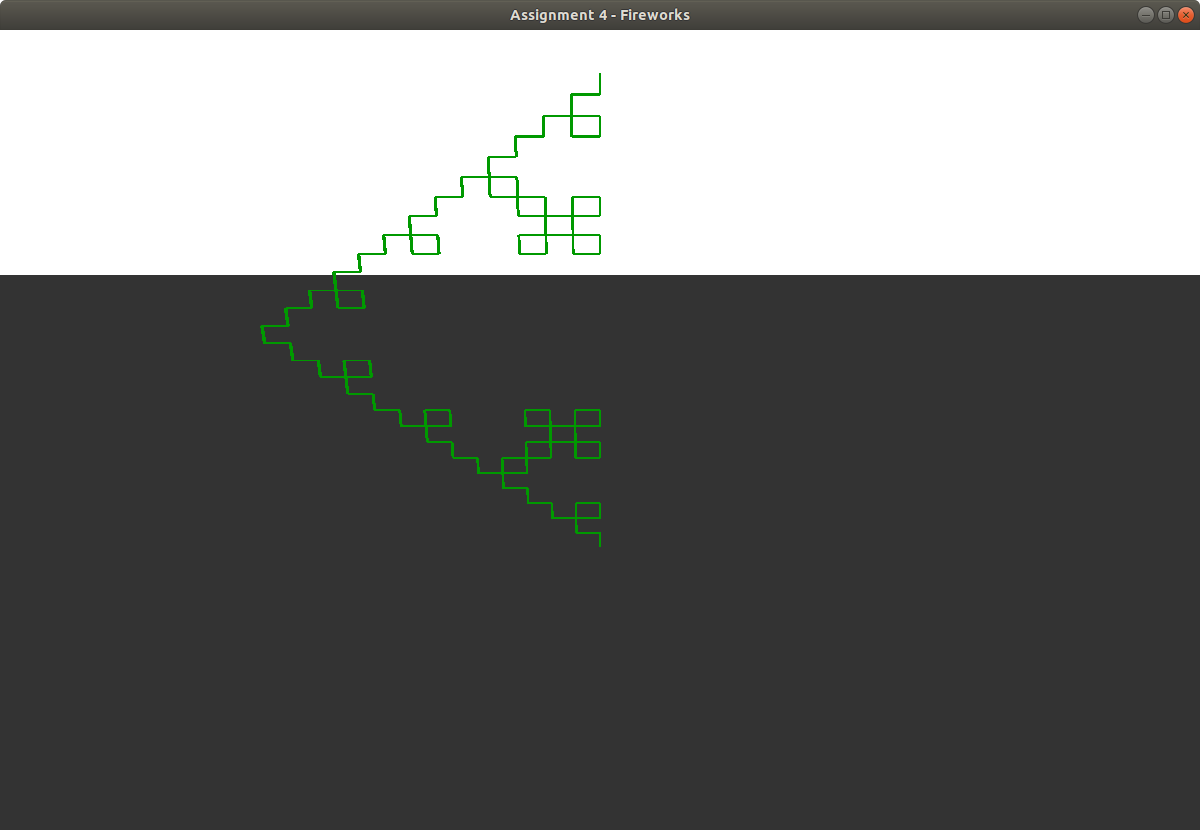
\includegraphics[scale=0.15]{KochCurve/KochCurve04.png}
		\caption{Koch Curve.}
	}
\end{figure}
\begin{figure}[htbp]
	\raggedright
	\textbf{\underline{Sierpinski Triangle:}} \\
	\#n = 4;\\
	\#define r 60;\\
	\#w : F(1);\\
	\#p1 : F(x) : * : X(x)-(r)F(x)-(r)X(x);\\
	\#p2 : X(x) : * : F(x)+(r)X(x)+(r)F(x);\\
	{\centering
		\vspace{7px}
		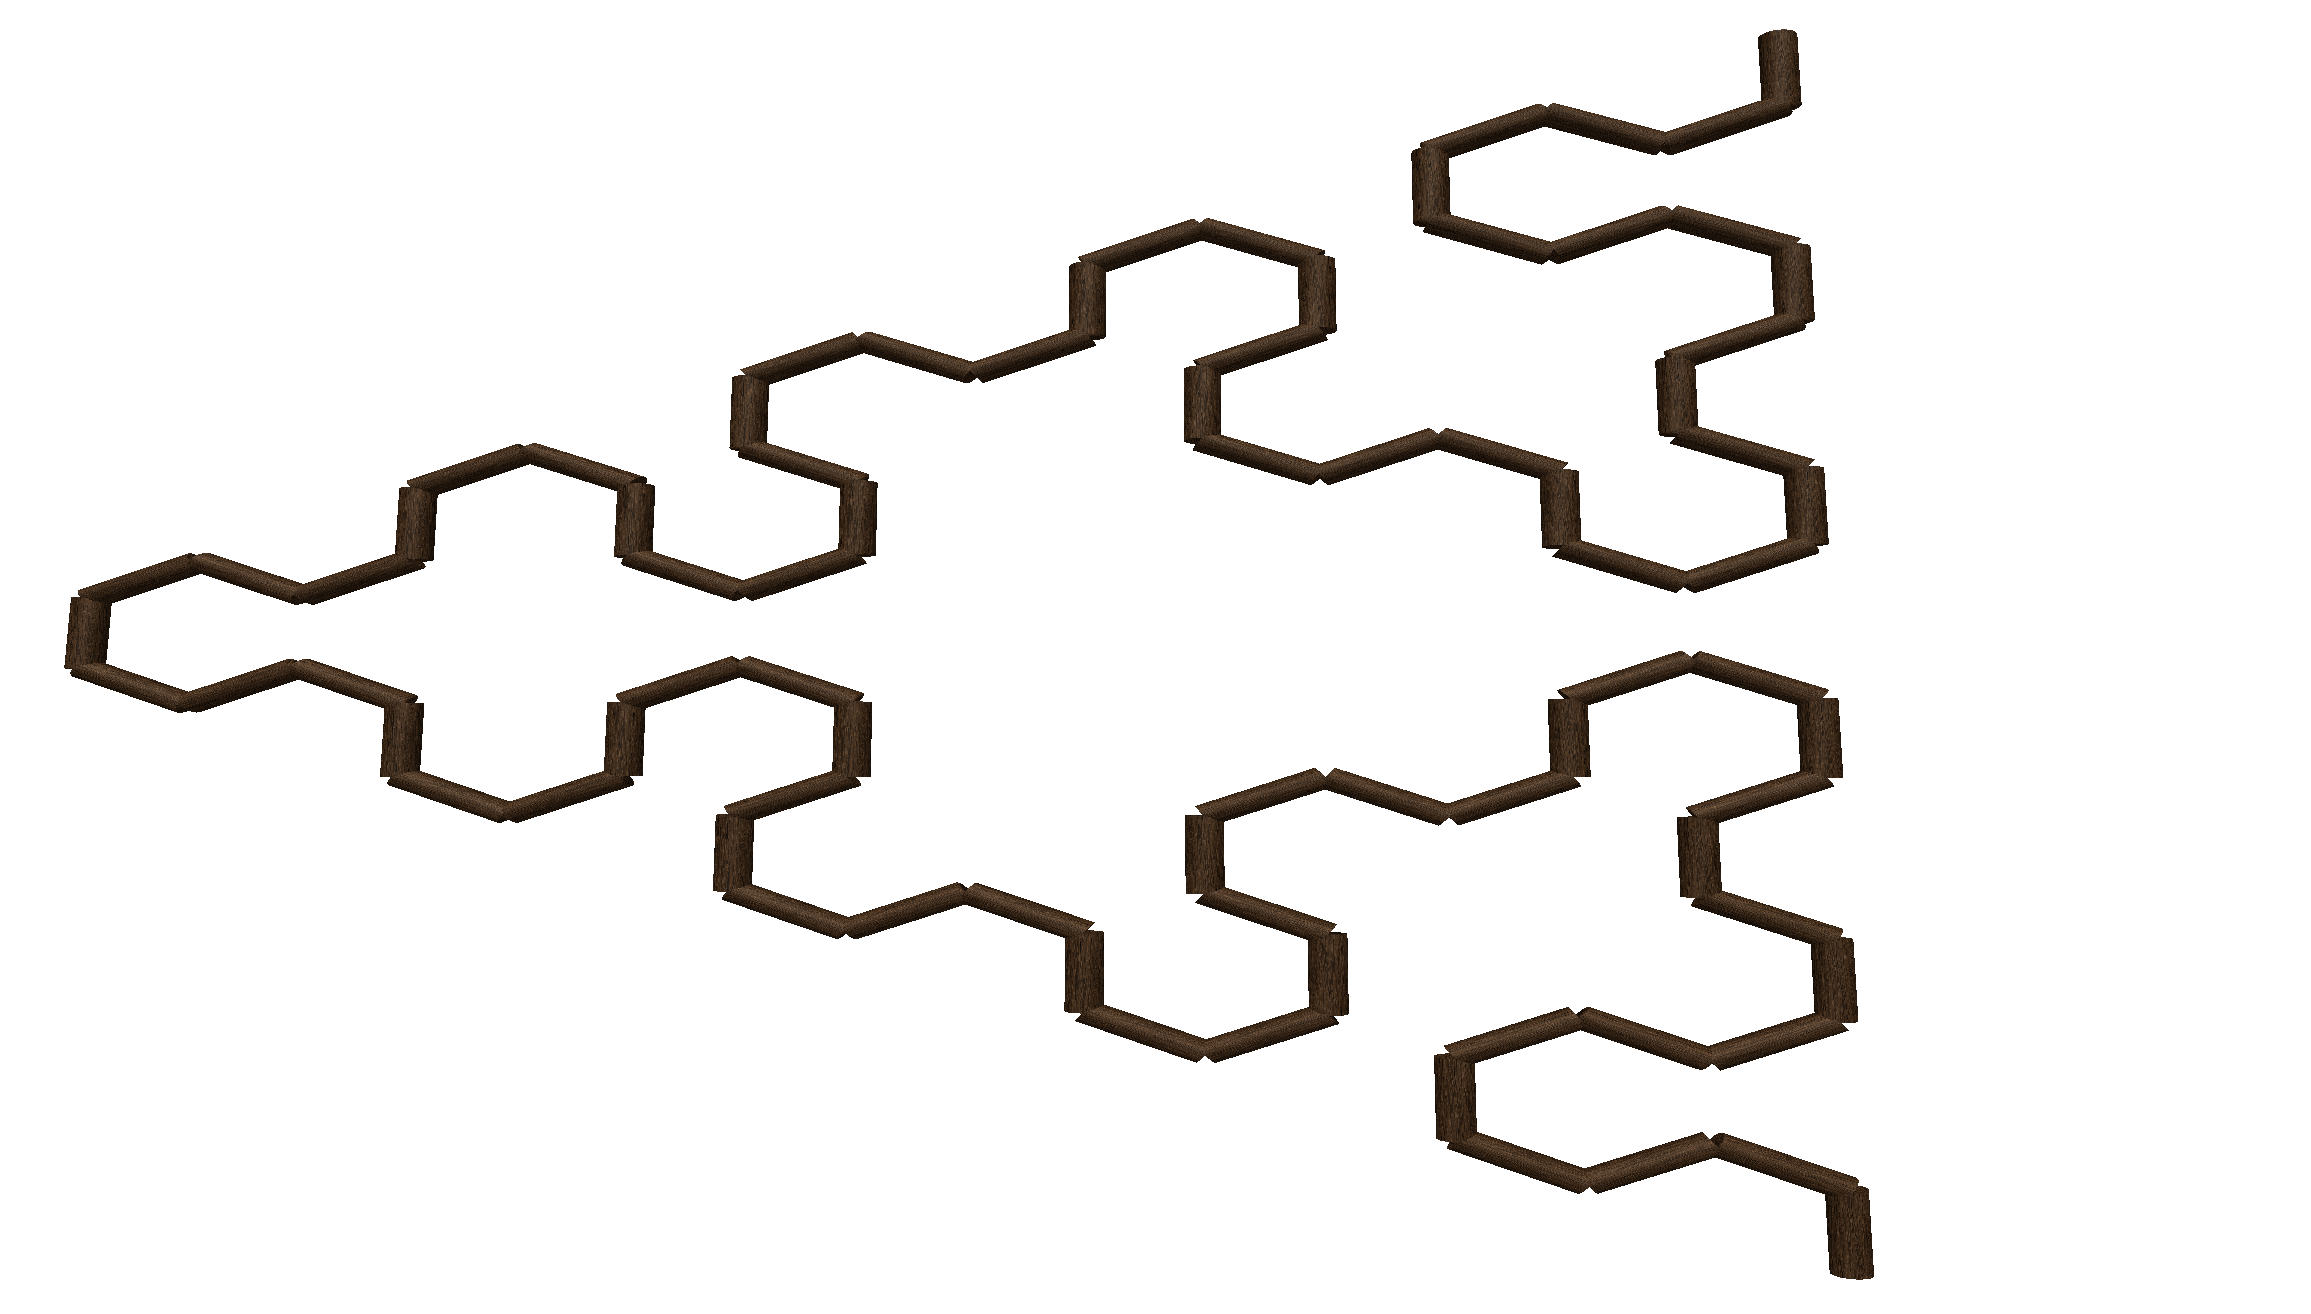
\includegraphics[scale=0.15]{SierpinskiTriangle/SierpinskiTriangle04.png}
		\caption{Sierpinski Triangle.}
	}
\end{figure}
\begin{figure}[htbp]
	\raggedright
	\textbf{\underline{Fractal Plant:}} \\
	\textbf{Alphabet:} X, F\\
	\textbf{Constants:} +, -, [, ] \\
	\textbf{Axiom:} X \\
	\textbf{Angle:} 25$^\circ$ \\
	\textbf{Rules:} \\
	X $\rightarrow$ F-[[X]+X]+F[+FX]-X\\
	F $\rightarrow$ FF \\
	{\centering
		\vspace{7px}
		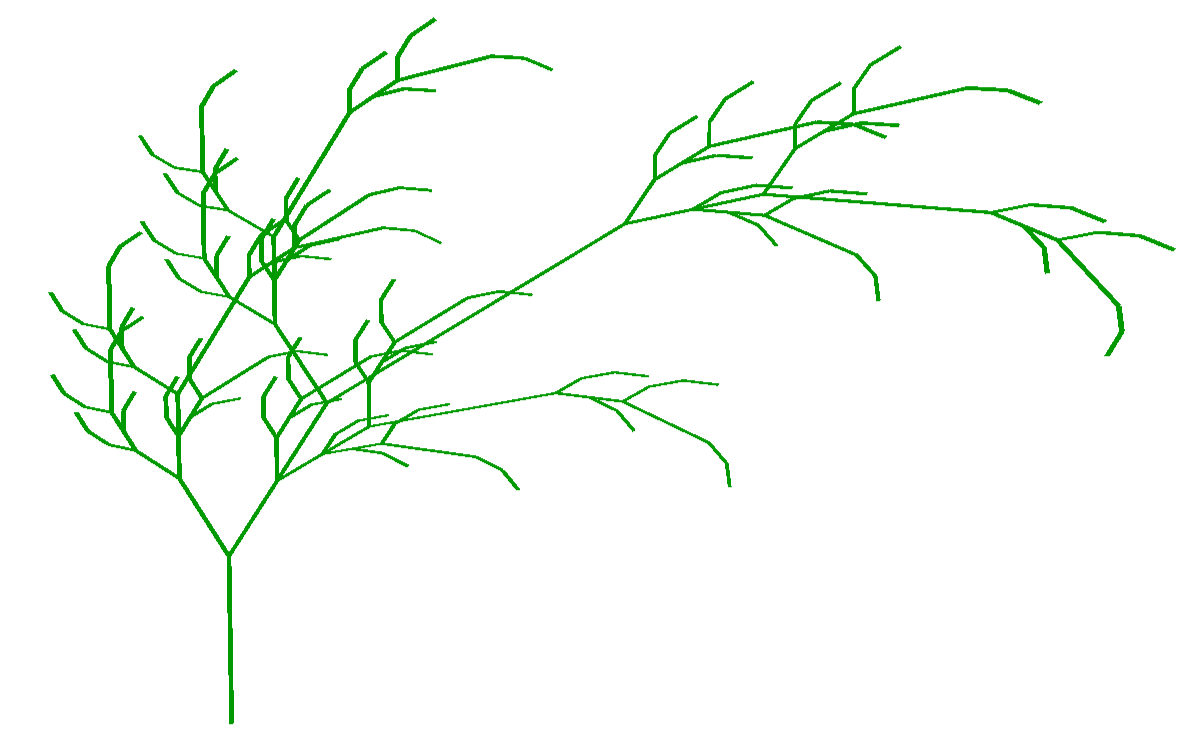
\includegraphics[scale=0.15]{FractalPlant/FractalPlant05.png}
		\caption{Fractal Plant.}
	}
\end{figure}
\begin{figure}[htbp]
	\raggedright
	\textbf{\underline{Fractal Bush:}} \\
	\textbf{Alphabet:} F\\
	\textbf{Constants:} +, -, [, ] \\
	\textbf{Axiom:} F \\
	\textbf{Angle:} 25$^\circ$ \\
	\textbf{Rules:} \\
	F $\rightarrow$ FF+[+F-F-F]-[-F+F+F]\\
	{\centering
		\vspace{7px}
		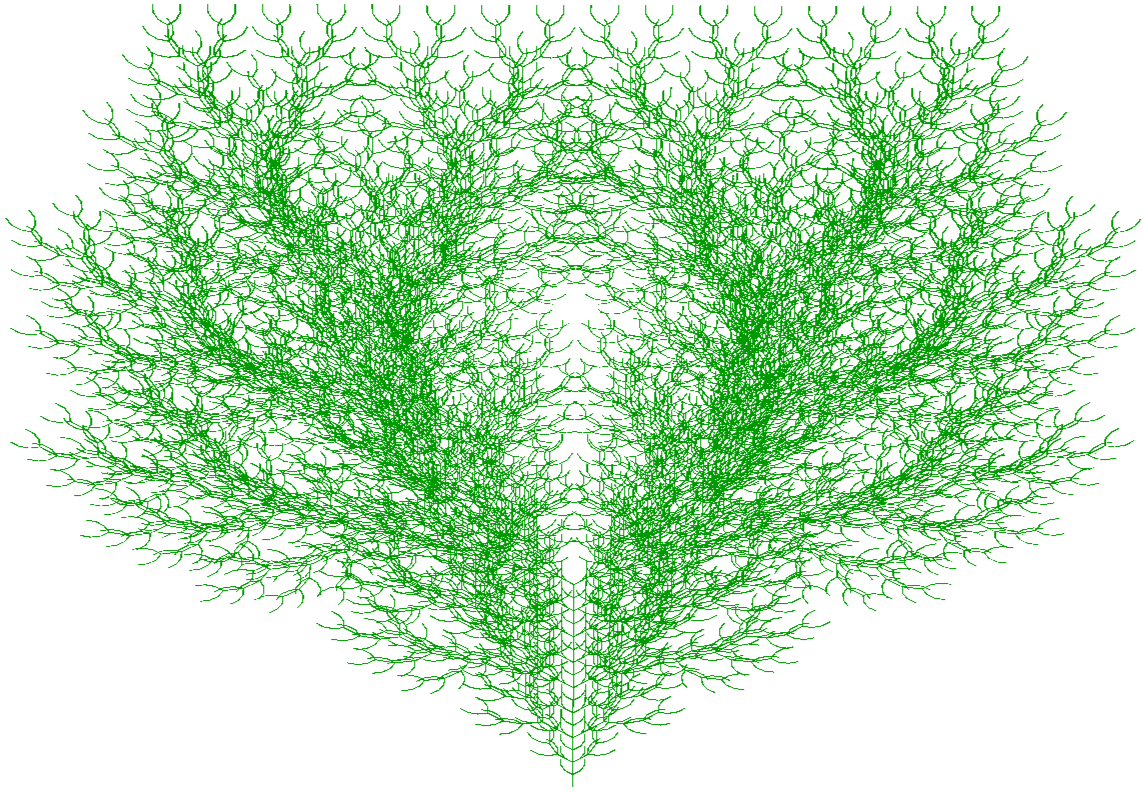
\includegraphics[scale=0.15]{FractalBush/FractalBush06.png}
		\caption{Fractal Bush.}
	}
\end{figure}

\FloatBarrier

\subsection{The Use of L-systems in 3D applications}

\begin{flushleft}

L-systems have been talked about and researched since its inception in 1968 by Aristid Lindenmayer. Over the years it's usefulness in modelling different types of plant life has been very clear, however its presence has been quite absent from any mainstream game engines for the most part, these engines relying either on digital artists skill to develop individual plants or on 3rd party software such as SpeedTree. These types of software use a multitude of different techniques however their methods are heavily rooted in Lindenmayer Systems. 

\end{flushleft}

\newpage

\section{Modeling Seamless Branches}

\begin{flushleft}

Modeling the branches of a plant is the most important part behind the overall look and feel of that plant. The L-system described in the previous sections is able to describe the most important details about the plants structure. For instance the width, length, weight and other important information. Our job now is to take this information and intelligently generate a model consisting of vertices, normals, texture coordinates and other information that can then be provided to the GPU and then rendered on the screen.\\

\vspace{5mm}

The most obvious way to generate a model for a branching structure would be to take a number of cylinders and to rotate and stack them according to the branching structure. In this way we are able to represent the overall branching structure of the tree. However there is a problem pointed out by Baele and Warz\'{e}e "The branches junction causes a continuity problem: to simply stack up cylinders generates a gap" \cite{baele2005real}. This can be shown in the figure below:

\FloatBarrier

\begin{figure}[htbp]
	{\centering
		\vspace{7px}
		\setlength{\fboxrule}{1pt}
		\fbox{
			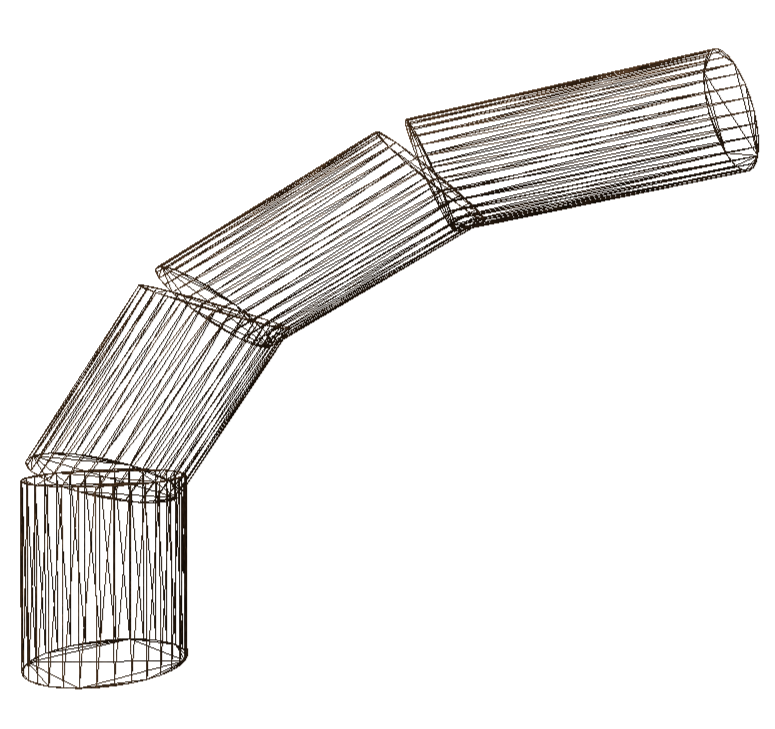
\includegraphics[scale=0.16]{Diagrams/stackedBranchesMesh.png}
		}
		\caption{Example of the continuity problem faced with stacked branching with a 25$^{\circ}$ bend per joint.}
	}
\end{figure}

\FloatBarrier

\vspace{5mm}


\vspace{5mm}

This simple method of stacking cylinders gives a reasonable looking tree structure and it is usually good enough when the angles of branches are not more than about 25$^{\circ}$ and the size of the branches do not change. However for a much more convincing tree structure we will want to do better than this. The logical next step would be to actively link the branch segments together.

\FloatBarrier

\begin{figure}[htbp]
	{\centering
		\vspace{7px}
		\setlength{\fboxrule}{1pt}
		\fbox{
			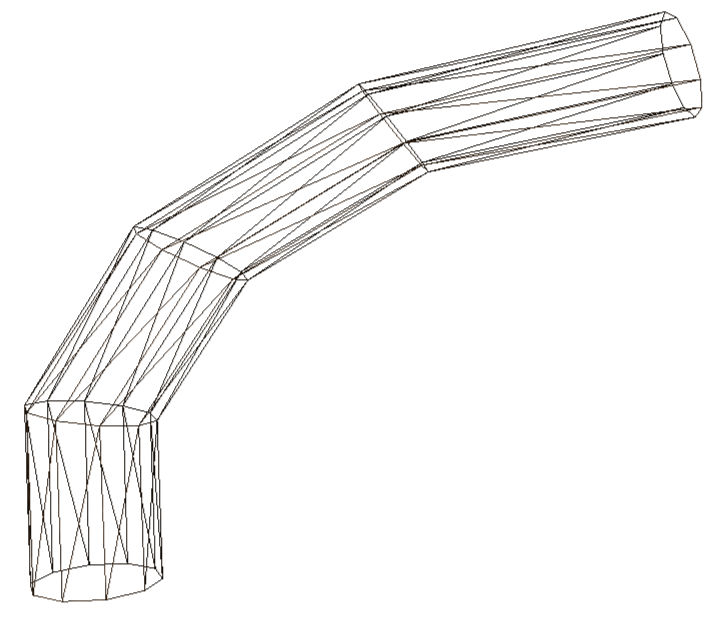
\includegraphics[scale=0.16]{Diagrams/linkedBranchesMesh.png}
		}
		\caption{Example of linked branching with a 25$^{\circ}$ bend per joint.}
	}
\end{figure}

\FloatBarrier

\end{flushleft}


